%# -*- coding: utf-8 -*-
% !TeX encoding = UTF-8 Unicode
% !TeX spellcheck = en_US
% !TeX TS-program = xelatex
%~ \XeTeXinputencoding "UTF-8"
% vim:ts=4:sw=4
%
% 以上设定默认使用 XeLaTex 编译,并指定 Unicode 编码,供 TeXShop 自动识别

%\documentclass[a4paper,10pt,twocolumn]{article}
\documentclass[letter,11pt,onecolumn]{book}
%\documentclass[letter,11pt,onecolumn,adobefonts]{ctexbook}

\newcommand{\doctitle}{Simulation framework}
\newcommand{\docauthor}{傅允辉}
\newcommand{\dockeywords}{Linux, Debian, Ubuntu, Networking, Home}
\newcommand{\docsubject}{}

\newcommand{\usedefaultTWO}[2]{
\if\relax\detokenize{#2}\relax
  #1
\else
  #2
\fi
}

\newcommand{\usedefaultTHREE}[3]{
\if\relax\detokenize{#3}\relax
  \usedefaultTWO{#1}{#2}
\else
  #3
\fi
}

% 用于接受从 xelatex/pdflatex 通过参数 -jobname 传入的参数来判定编译何种语言的版本。
% \cnt 的三个参数分别为 en/zh/tw 的内容
\newcommand{\cnt}[3]{{#1}{#2}{#3}}
%\newcommand{\cnt}[3]{#1} % default en
\usepackage{ifthen}
\ifthenelse{\equal{\detokenize{lang-zh}}{\jobname}}{
  \renewcommand{\cnt}[3]{\usedefaultTWO{#1}{#2}}
}{
  \ifthenelse{\equal{\detokenize{lang-tw}}{\jobname}}{
    \renewcommand{\cnt}[3]{\usedefaultTHREE{#1}{#2}{#3}}
  }{
    % default en
    \renewcommand{\cnt}[3]{#1}
    %\renewcommand{\cnt}[3]{#2}
  }
}

\newcommand{\cnts}[3]{{#1} {#2}}

% 根据配置来设置中文环境
\newcommand\usefontspeczh[1]{#1} % use fontspec for zh_CN
\newcommand\charsetzhcn[1]{#1} % the charset encoding for zh_CN
\newcommand\formatzhcn[1]{#1} % the page format for zh_CN
\cnt{
\renewcommand\usefontspeczh[1]{}
\renewcommand\charsetzhcn[1]{}
\renewcommand\formatzhcn[1]{}
}{
%\renewcommand\usefontspeczh[1]{}
%\renewcommand\charsetzhcn[1]{}
%\renewcommand\formatzhcn[1]{}
}{
%\renewcommand\usefontspeczh[1]{}
%\renewcommand\charsetzhcn[1]{}
%\renewcommand\formatzhcn[1]{}
}
%# -*- coding: utf-8 -*-
% !TeX encoding = UTF-8 Unicode
% !TeX spellcheck = en_US
% !TeX TS-program = xelatex
%~ \XeTeXinputencoding "UTF-8"
% vim:ts=4:sw=4
%
% 以上设定默认使用 XeLaTex 编译,并指定 Unicode 编码,供 TeXShop 自动识别

% 使用 LaTex 写中文的配置模板
%\documentclass[12pt]{article}

%\newcommand{\doctitle}{Peer-to-Peer Communication Across Network Address Translators}
%\newcommand{\doctitle}{穿越NAT的点对点通信}
%\newcommand{\docauthor}{Bryan Ford \& Pyda Srisuresh \& Dan Kegel}
%\newcommand{\dockeywords}{NAT穿越, 点对点, NAT Traversal, Peer-to-Peer}
%\newcommand{\docsubject}{NAT穿越}
%\newcommand\usefontspeczh[1]{#1} % use fontspec for zh_CN
%\newcommand\charsetzhcn[1]{#1} % the charset encoding for zh_CN
%\newcommand\formatzhcn[1]{#1} % the page format for zh_CN

\newcommand\mymainfont{DejaVu Serif}%{Times New Roman} %{DejaVu Serif}
\newcommand\mymonofont{DejaVu Sans Mono}%{FreeMono} %{WenQuanYi Micro Hei Mono} %{Monaco}
\newcommand\myboldfont{WenQuanYi Micro Hei Mono}%{AR PL UKai CN}%{YaHei Consolas Hybrid}%{黑体}%{標楷體}
\newcommand\mysansfont{DejaVu Sans}%{FreeSans}
\newcommand\myitalicfont{DejaVu Serif}%{Times New Roman} %{Garamond}

\newcommand\mycjkboldfont{WenQuanYi Micro Hei Mono}%{Adobe Heiti Std}%{AR PL UKai CN}%{YaHei Consolas Hybrid}%{黑体}%{標楷體}
\newcommand\mycjkitalicfont{全字庫正楷體} %{Adobe Kaiti Std}
\newcommand\mycjkmainfont{AR PL UMing CN}%{Adobe Song Std}%{仿宋}%{宋体}%{新宋体}%{文鼎PL新宋}%
\newcommand\mycjksansfont{Adobe Ming Std}
\newcommand\mycjkmonofont{WenQuanYi Micro Hei Mono}%{AR PL UMing CN}%{WenQuanYi Micro Hei Mono}

\usepackage{ifthen}
\usepackage{ifpdf}
\usepackage{ifxetex}
\usepackage{ifluatex}

\usepackage{color}
\usepackage[rgb,x11names]{xcolor} %must before tikz, x11names defines RoyalBlue3


\usefontspeczh{

\usepackage[cm-default]{fontspec} % XeLaTex 配合 fontspec

\charsetzhcn{
  %\renewcommand\mycjkmainfont{AR PL UMing CN}%{仿宋}%{宋體}%{新宋體}%{文鼎PL新宋}%

  \ifxetex    % xelatex

    %\usepackage[cm-default]{fontspec} % XeLaTex 配合 fontspec 可以非常方便地设置字体。[cm-default]选项主要用来解决使用数学环境时数学符号不能正常显示的问题
    %\usepackage{xltxtra,xunicode} %这行和上行 \usepackage[cm-default]{fontspec} 解决公式不正常的问题.但是打开后有些如 itemize 的点不能显示。

    \usepackage[
        BoldFont, % 允許粗體
        SlantFont,        % 允許斜體
        %CJKsetspaces,
        CJKchecksingle
        ]{xeCJK}
    \defaultfontfeatures{Mapping=tex-text} %如果沒有它,會有一些 tex 特殊字符無法正常使用,比如連字符。

    \XeTeXlinebreaklocale "zh"                      % 重要,使得中文可以正確斷行!
    \XeTeXlinebreakskip = 0pt plus 1pt minus 0.1pt  %

    \setCJKmainfont[BoldFont=\mycjkboldfont, ItalicFont=\mycjkitalicfont]{\mycjkmainfont}
    \setCJKsansfont{\mycjksansfont}%{Adobe Ming Std} %{AR PL UMing CN} %{Microsoft YaHei}
    \setCJKmonofont{\mycjkmonofont}

  \fi


\formatzhcn{
    %\newfontfamily{\j}{Osaka}       % 设置特殊字符,这里是为日文准备的特殊字体。没有该字体,所以关闭。

    \setlength{\parindent}{2.04em}  %设置首行缩进。只有中文才打开。
    \linespread{1.3}                % 设置行距

    %\definecolor{bisque}{rgb}{.996,.891,.755}
    %\pagecolor{bisque} % 设置背景颜色

    % 设置原文照排环境的字体
    \makeatletter
    \def\verbatim@font{\sffamily\small}
    \makeatother

    % 将默认的英文重定义为中文
    \renewcommand{\contentsname}{\cnt{Content}{目录}{目錄}}
    \renewcommand{\listfigurename}{\cnt{List of Figures}{插图目录}{插圖目錄}}
    \renewcommand{\listtablename}{\cnt{List of Tables}{表格目录}{表格目錄}}
    \renewcommand{\indexname}{\cnt{Index}{索引}{索引}}
    \renewcommand{\tablename}{\cnt{Table}{表}{表}}
    \renewcommand{\figurename}{\cnt{Figure}{图}{圖}}
    \renewcommand{\appendixname}{\cnt{Chapter}{附录}{附錄}}

    % article
    %\renewcommand{\refname}{\cnt{Bibliography}{参考文献}{參考文獻}}
    %\renewcommand{\abstractname}{\cnt{Abstract}{摘要}{摘要}}

    % book
    %\renewcommand{\chaptername}{\cnt{Chapter}{章节}{章節}}
    %\renewcommand{\bibname}{\cnt{Bibliography}{参考}{參考}}

    %\renewcommand{\IEEEkeywordsname}{\cnt{Keywords}{关键词}{關鍵詞}}


    % 设置页眉页脚
    \usepackage[pagestyles,compact]{titlesec} % 定制页眉页脚
    \newpagestyle{main}{%
        \sethead[$\cdot$~\thepage~$\cdot$][][\thesection\quad%
        \sectiontitle]{\thesection\quad\sectiontitle}{}{%
            $\cdot$~\thepage~$\cdot$}
        \setfoot{}{}{}\headrule}
        \pagestyle{main}
        \renewpagestyle{plain}{\sethead{}{}{}\setfoot{}{}{}}
    \pagestyle{plain}

    %% 设置chapter, section与subsection的格式
    \titleformat{\chapter}{\centering\huge}{\textbf{第\thechapter{}章}}{1em}{\textbf}
    \titleformat{\section}{\centering\LARGE}{\textbf{\thesection}}{1em}{\textbf}
    \titleformat{\subsection}{\Large}{\textbf{\thesubsection}}{1em}{\textbf}

    %% For LaN
    \newcommand{\LaN}{L{\scriptsize\hspace{-0.47em}\raisebox{0.23em}{A}}\hspace{-0.1em}N}

    %% 去掉表头中的冒号
    \makeatletter
        \long\def\@makecaption#1#2{%
            \vskip\abovecaptionskip
            \sbox\@tempboxa{#1~~#2}%
            \ifdim \wd\@tempboxa >\hsize
                #1~~#2\par
            \else
                \global \@minipagefalse
                \hb@xt@\hsize{\hfil\box\@tempboxa\hfil}%
            \fi
            \vskip\belowcaptionskip}
    \makeatother
} % formatzhcn

} % \charsetzhcn

\setmonofont[Scale=0.8]{\mymonofont} % 英文等宽字体
\setsansfont{\mysansfont}       % 英文无衬线字体
%\setmainfont{\mymainfont}        % 英文衬线字体, setmainfont=setromanfont
\setromanfont[Mapping=tex-text,  % 沿用 LaTex 的一些习惯的标点转换,例如 en-dash 以两个减号表示
    Ligatures={Required,Common}, % 如果此字体内置 Ligatures 定义则启用
    ItalicFont={\myitalicfont},  % 斜体用 Times Italic,严格来说只有拉丁子母有斜体。
    BoldFont={\myboldfont}]      % 粗体用字体
    {\mymainfont}                % 内文使用字体, Linux 下用 "fc-list :lang=zh-cn" 列出支持的中文字体
} % \usefontspeczh

% 设置中文状态下, 恢复 lstlisting 的 mono 字体
\usepackage[T1]{fontenc}
\DeclareTextCommandDefault{\nobreakspace}{\leavevmode\nobreak\ } % EU1 encoding setup has changed \nobreakspace from being an encoding-independent command to an encoding-dependent command, but without setting up a default definition so it works in all encodings.

\usepackage{dtklogos} % \LaTeXe 等
% XeTeX logo
%\def\XeTeX{\leavevmode
%    \setbox0=\hbox{X\lower.5ex\hbox{\kern-.15em\reflectbox{E}}\kern-.1667em \TeX}%
%    \dp0=0pt\ht0=0pt\box0}

% the algorithm2e package
\makeatletter
\newif\if@restonecol
\makeatother
\let\algorithm\relax
\let\endalgorithm\relax
\usepackage[ruled,vlined]{algorithm2e} %\usepackage[figure,ruled,vlined]{algorithm2e}

\usepackage{url}
\usepackage{array}

\usepackage{courier}
\usepackage{listings} % list the source code
\definecolor{ForestGreen}{rgb}{0.13,0.55,0.13}

\lstset{
    language=C,
    captionpos=b, %t,
    tabsize=3,
    basicstyle=\footnotesize\ttfamily, %basicstyle=\ttfamily\normalsize, %basicstyle=\small\ttfamily, %\normalfont\ttfamily, % \large\ttfamily, % \small\ttfamily, % \footnotesize\ttfamily, % \scriptsize\ttfamily, % Standardschrift,
    numbers=left,               %左侧显示行号 往左靠,还可以为right,或none,即不加行号
    stepnumber=1,               %若设置为2,则显示行号为1,3,5,即stepnumber为公差,默认stepnumber=1
    %numberstyle=\tiny,         %行号字体用小号
    numberstyle={\color[RGB]{0,192,192}\tiny} ,%设置行号的大小,大小有tiny,scriptsize,footnotesize,small,normalsize,large等
    numbersep=8pt,              %设置行号与代码的距离,默认是5pt
    breaklines=true,            %对过长的代码自动换行
    showstringspaces=false,     %不显示代码字符串中间的空格标记
    frame=shadowbox, %=lines,                    %把代码用带有阴影的框圈起来
    stringstyle=\ttfamily,      % 代码字符串的特殊格式
    commentstyle=\color{ForestGreen}, %\color{red!50!green!50!blue!50}, %浅灰色的注释
    rulesepcolor=\color{red!20!green!20!blue!20}, %代码块边框为淡青色
    keywordstyle=\color{blue!90}\bfseries,        %代码关键字的颜色为蓝色,粗体
    backgroundcolor=\color[rgb]{1,1,1},%\color[RGB]{245,245,244},   %代码背景色 \color[rgb]{0.91,0.91,0.91}
    framextopmargin=2pt,framexbottommargin=2pt,abovecaptionskip=-3pt,belowcaptionskip=3pt,
%    xleftmargin=4em,xrightmargin=4em, % 设定listing左右的空白
%    %language={[ISO]C++},       %language为,还有{[Visual]C++}
%    alsolanguage=Java,
%    %alsolanguage=[ANSI]C,      %可以添加很多个alsolanguage,如alsolanguage=matlab,alsolanguage=VHDL等
%    %alsolanguage= tcl,
%    alsolanguage= XML,
%    keepspaces=true,            %
%    breakindent=22pt,           %
%    breakindent=4em,            %
%    showspaces=false,           %
%    flexiblecolumns=true,       %
%    breakautoindent=true,       %
%    aboveskip=1em,              %代码块边框
%    %% added by http://bbs.ctex.org/viewthread.php?tid=53451
%    fontadjust,
%    texcl=true,
%    escapeinside=``,            %在``里显示中文
%    %escapebegin=\begin{CJK*}{GBK}{hei},escapeend=\end{CJK*},
%    % 设定中文冲突,断行,列模式,数学环境输入,listing数字的样式
%    extendedchars=false,columns=flexible,
%    mathescape=false,
%    % numbersep=-1em,
    emph={label}
}

\renewcommand{\ttdefault}{pcr}

\definecolor{darkgreen}{cmyk}{0.7, 0, 1, 0.5}
\definecolor{darkblue}{rgb}{0.1, 0.1, 0.5}
\lstdefinelanguage{diff}
{
    keywords={+, -, \ , @@, diff, index, new},
    sensitive=false,
    morecomment=[l][""]{\ },
    morecomment=[l][\color{darkgreen}]{+},
    morecomment=[l][\color{red}]{-},
    morecomment=[l][\color{darkblue}]{@@},
    morecomment=[l][\color{darkblue}]{diff},
    morecomment=[l][\color{darkblue}]{index},
    morecomment=[l][\color{darkblue}]{new},
    morecomment=[l][\color{darkblue}]{similarity},
    morecomment=[l][\color{darkblue}]{rename},
}

\lstdefinelanguage{JavaScript}{
  keywords={typeof, new, true, false, catch, function, return, null, catch, switch, var, if, in, while, do, else, case, break},
  keywordstyle=\color{blue}\bfseries,
  ndkeywords={class, export, boolean, throw, implements, import, this},
  ndkeywordstyle=\color{darkgray}\bfseries,
  identifierstyle=\color{black},
  sensitive=false,
  comment=[l]{//},
  morecomment=[s]{/*}{*/},
  %commentstyle=\color{purple}\ttfamily,
  commentstyle=\color{green}\ttfamily,
  stringstyle=\color{red}\ttfamily,
  morestring=[b]',
  morestring=[b]"
}

\usepackage{tabularx} % long table
\usepackage{booktabs,longtable} % table in seperate pages.


\ifxetex % xelatex
\else
    %The cmap package is intended to make the PDF files generated by pdflatex "searchable and copyable" in acrobat reader and other compliant PDF viewers.
    \usepackage{cmap}%
\fi
% ============================================
% Check for PDFLaTeX/LaTeX
% ============================================
\newcommand{\outengine}{xetex}
\newif\ifpdf
\ifx\pdfoutput\undefined
  \pdffalse % we are not running PDFLaTeX
  \ifxetex
    \renewcommand{\outengine}{xetex}
  \else
    \renewcommand{\outengine}{dvipdfmx}
  \fi
\else
  \pdfoutput=1 % we are running PDFLaTeX
  \pdftrue
  \usepackage{thumbpdf}
  \renewcommand{\outengine}{pdftex}
  \pdfcompresslevel=9
\fi
\usepackage[\outengine,
    bookmarksnumbered, %dvipdfmx
    %% unicode, %% 不能有unicode选项,否则bookmark会是乱码
    colorlinks=true,
    citecolor=red,
    urlcolor=blue,        % \href{...}{...} external (URL)
    filecolor=red,      % \href{...} local file
    linkcolor=black, % \ref{...} and \pageref{...}
    breaklinks,
    pdftitle={\doctitle},
    pdfauthor={\docauthor},
    pdfsubject={\docsubject},
    pdfkeywords={\dockeywords},
    pdfproducer={Latex with hyperref},
    pdfcreator={pdflatex},
    %%pdfadjustspacing=1,
    pdfborder=1,
    pdfpagemode=UseNone,
    pagebackref,
    bookmarksopen=true]{hyperref}

% --------------------------------------------
% Load graphicx package with pdf if needed 
% --------------------------------------------
\ifxetex    % xelatex
    \usepackage{graphicx}
\else
    \ifpdf
        \usepackage[pdftex]{graphicx}
        \pdfcompresslevel=9
    \else
        \usepackage{graphicx} % \usepackage[dvipdfm]{graphicx}
    \fi
\fi

%% \DeclareGraphicsRule{.jpg}{eps}{.bb}{}
%% \DeclareGraphicsRule{.png}{eps}{.bb}{}
\graphicspath{{./} {figures/}}
\usepackage{flafter} % 防止图形在文字前

%%%% 字体:
%Adobe Heiti Std 和 Adobe Song Std是砖头公司出的两款超pp的字体,有人把它们用在latex排版中,效果超级好。
%windows版在 Program Files/Adobe/Acrobat 8.0/Resource/CIDFont 下。

%sudo mkdir /usr/share/fonts/adobe
%sudo cp DIR2adobefonts/*.otf /usr/share/fonts/adobe
%sudo chmod 644 /usr/share/fonts/adobe/*.otf # 当前用户读写,当前组用户读写,其他用户只读

%cd /usr/share/fonts/adobe/
%sudo mkfontscale #(创建fonts.scale文件,控制字体旋转缩放)
%sudo mkfontdir #(创建fonts.dir文件,控制字体粗斜体产生)
%sudo fc-cache -fv # (建立字体缓存信息,也就是让系统认识认识)
%fc-list :lang=zh-cn # 看看装上没


%安装 LaTeX+XeTeX环境的过程, 你也使用Emacs来编辑TeX文件的话, 那么一定要安上AUCTeX这个扩展
%sudo apt-get install texlive texlive-latex-extra texlive-xetex lmodern # 首先是LaTeX与XeTeX的安装

%sudo apt-get install auctex

%安装好以后, 重点是配置.emacs文件, 因为AUCTeX本身是不支持通过xelatex编译的.
%;; AUCTeX
%(defun auctex ()
  %(add-to-list 'TeX-command-list '("XeLaTeX" "%`xelatex%(mode)%' %t; %`xelatex%(mode)%' %t" TeX-run-TeX nil t)) ;; 这里我编译了两次
    %(setq TeX-command-default "XeLaTeX") ;; 设定默认编译命令为XeLaTeX
    %(setq TeX-save-query nil)            ;; 保存之前不询问
    %(setq TeX-show-compilation t))       ;; 在新窗口显示编译过程
%(add-hook 'LaTeX-mode-hook 'auctex)

%(custom-set-variables
 %'(TeX-output-view-style (quote (("^dvi$nnnnnnn" ("^landscape$" "^pstricks$\\|^pst-\\|^psfrag$") "%(o?)dvips -t landscape %d -o && gv %f") ("^dvi$" "^pstricks$\\|^pst-\\|^psfrag$" "%(o?)dvips %d -o && gv %f") ("^dvi$" ("^a4\\(?:dutch\\|paper\\|wide\\)\\|sem-a4$" "^landscape$") "%(o?)xdvi %dS -paper a4r -s 0 %d") ("^dvi$" "^a4\\(?:dutch\\|paper\\|wide\\)\\|sem-a4$" "%(o?)xdvi %dS -paper a4 %d") ("^dvi$" ("^a5\\(?:comb\\|paper\\)$" "^landscape$") "%(o?)xdvi %dS -paper a5r -s 0 %d") ("^dvi$" "^a5\\(?:comb\\|paper\\)$" "%(o?)xdvi %dS -paper a5 %d") ("^dvi$" "^b5paper$" "%(o?)xdvi %dS -paper b5 %d") ("^dvi$" "^letterpaper$" "%(o?)xdvi %dS -paper us %d") ("^dvi$" "^legalpaper$" "%(o?)xdvi %dS -paper legal %d") ("^dvi$" "^executivepaper$" "%(o?)xdvi %dS -paper 7.25x10.5in %d") ("^dvi$" "." "%(o?)xdvi %dS %d") ("^pdf$" "." "acroread %o %(outpage)") ("^html?$" "." "netscape %o")))))

%最后那个有点长, 主要是没有找到合适的方法像添加XeLaTeX一样只需要写新增的条目, 所以这里就把原有的和修改以后的都写了出来. 其实只改了一个地方, 已经用蓝色标注出来了, 就是在使用C-c C-v预览PDF文件的时候使用什么软件来打开. 我这里就是acroread, 你用的其它的话, 可以相应修改.
%这样修改好以后, 以后就可以直接使用C-c C-c编译, C-c C-v预览, C-c `在错误间跳转了.

%但是TeX Live中的install-info文件会导致源安装AUCTeX的时候失败, 所以如果是先安装的TeX Live, 再安装AUCTeX, 就需要先把TeX Live的install-info"消灭"掉: 
%sudo mv /usr/local/bin/install-info /usr/local/bin/install-info.bak

%-------------------------------------------------------------------
%终于搞定在emacs+auctex中设置xelatex为默认编译命令!

%只要在在~/.emacs中加上

%(add-hook 'LaTeX-mode-hook (lambda()
    %(add-to-list 'TeX-command-list '("XeLaTeX" "%`xelatex%(mode)%' %t" TeX-run-TeX nil t))
    %(setq TeX-command-default "XeLaTeX")
    %(setq TeX-save-query  nil )
    %(setq TeX-show-compilation t)
    %))

%第一行参考auctex的手册auctex.pdf,版本是11.84 ;
%(add-to-list 'TeX-command-list '("XeLaTeX" "%`xelatex%(mode)%' %t" TeX-run-TeX nil t)) 会在Command 这一栏中增加了XeLaTeX这一项命令;
%(setq TeX-command-default "XeLaTeX")  则使得以后用C-c C-c就是默认用xelatex 命令编译tex文档;
%(setq TeX-save-query  nil ) 这一行不用确认保存就开始执行编译;
%(setq TeX-show-compilation t)  这一行是看到编译的滚动信息。
%现在还是在latex-mode下配置,下一步看能否在pdflatex-mode 下配置。


%(add-to-list 'TeX-command-list '("XeLaTeX" "%`xelatex%(mode)%' %t" TeX-run-TeX nil t)) 这一行中的"%`xelatex%(mode)%' %t"
%写成"xelatex  %t" 已经可以了。



\newcommand\comments[1]{#1}
\renewcommand\comments[1]{}

\usepackage{xcolor}

\usepackage{amssymb}
%\usepackage{amsmath,amsfonts,amsthm}

\usepackage{array}
% table's multirow and multicolumn
\usepackage{multirow}

\usepackage{chapterbib}
\usepackage[sectionbib,super,square,sort&compress]{natbib}

%\usepackage[margin=1.8cm,nohead]{geometry}
\usepackage[margin=0.8in,nohead]{geometry}
%\usepackage[top=1in,bottom=1in,left=1.25in,right=1.25in]{geometry} % 设置页边距
%\setlength{\belowcaptionskip}{1em} % 设置caption之后的距离

%opening
\title{\doctitle}
\author{\docauthor}
%\date{2014-03}

\begin{document}

\maketitle
\tableofcontents

%# -*- coding: utf-8 -*-
% !TeX encoding = UTF-8 Unicode
% !TeX spellcheck = en_US
% !TeX TS-program = xelatex
%~ \XeTeXinputencoding "UTF-8"
% vim:ts=4:sw=4
%
% 以上设定默认使用 XeLaTex 编译,并指定 Unicode 编码,供 TeXShop 自动识别

\chapter{High Level Design}



\begin{enumerate}
  \item 使用 flowchart 将处理流程初步理清
  \item 使用 \href{http://www.cascading.org/}{Cascading}/MapReduce 实现系统
  \item 测试
\end{enumerate}


\section{介绍}

\begin{enumerate}
  \item simulation task:
  generate the NS2 TCL scripts, and run ns2

  \item plotting figures:
  
\end{enumerate}


\section{整体结构}
图 \ref{fig:system} 是整个系统的运行框架。

\definecolor{vidtransoriginfile}{HTML}{D7FE39}
\definecolor{vidtranstmpfile}{HTML}{EDE80F}
\definecolor{vidtransfinalfile}{HTML}{FFE985}
\definecolor{vidtransprocess}{HTML}{FEA93E}
\definecolor{vidtransfuncio}{HTML}{DADAFF}
\begin{figure}\centering
  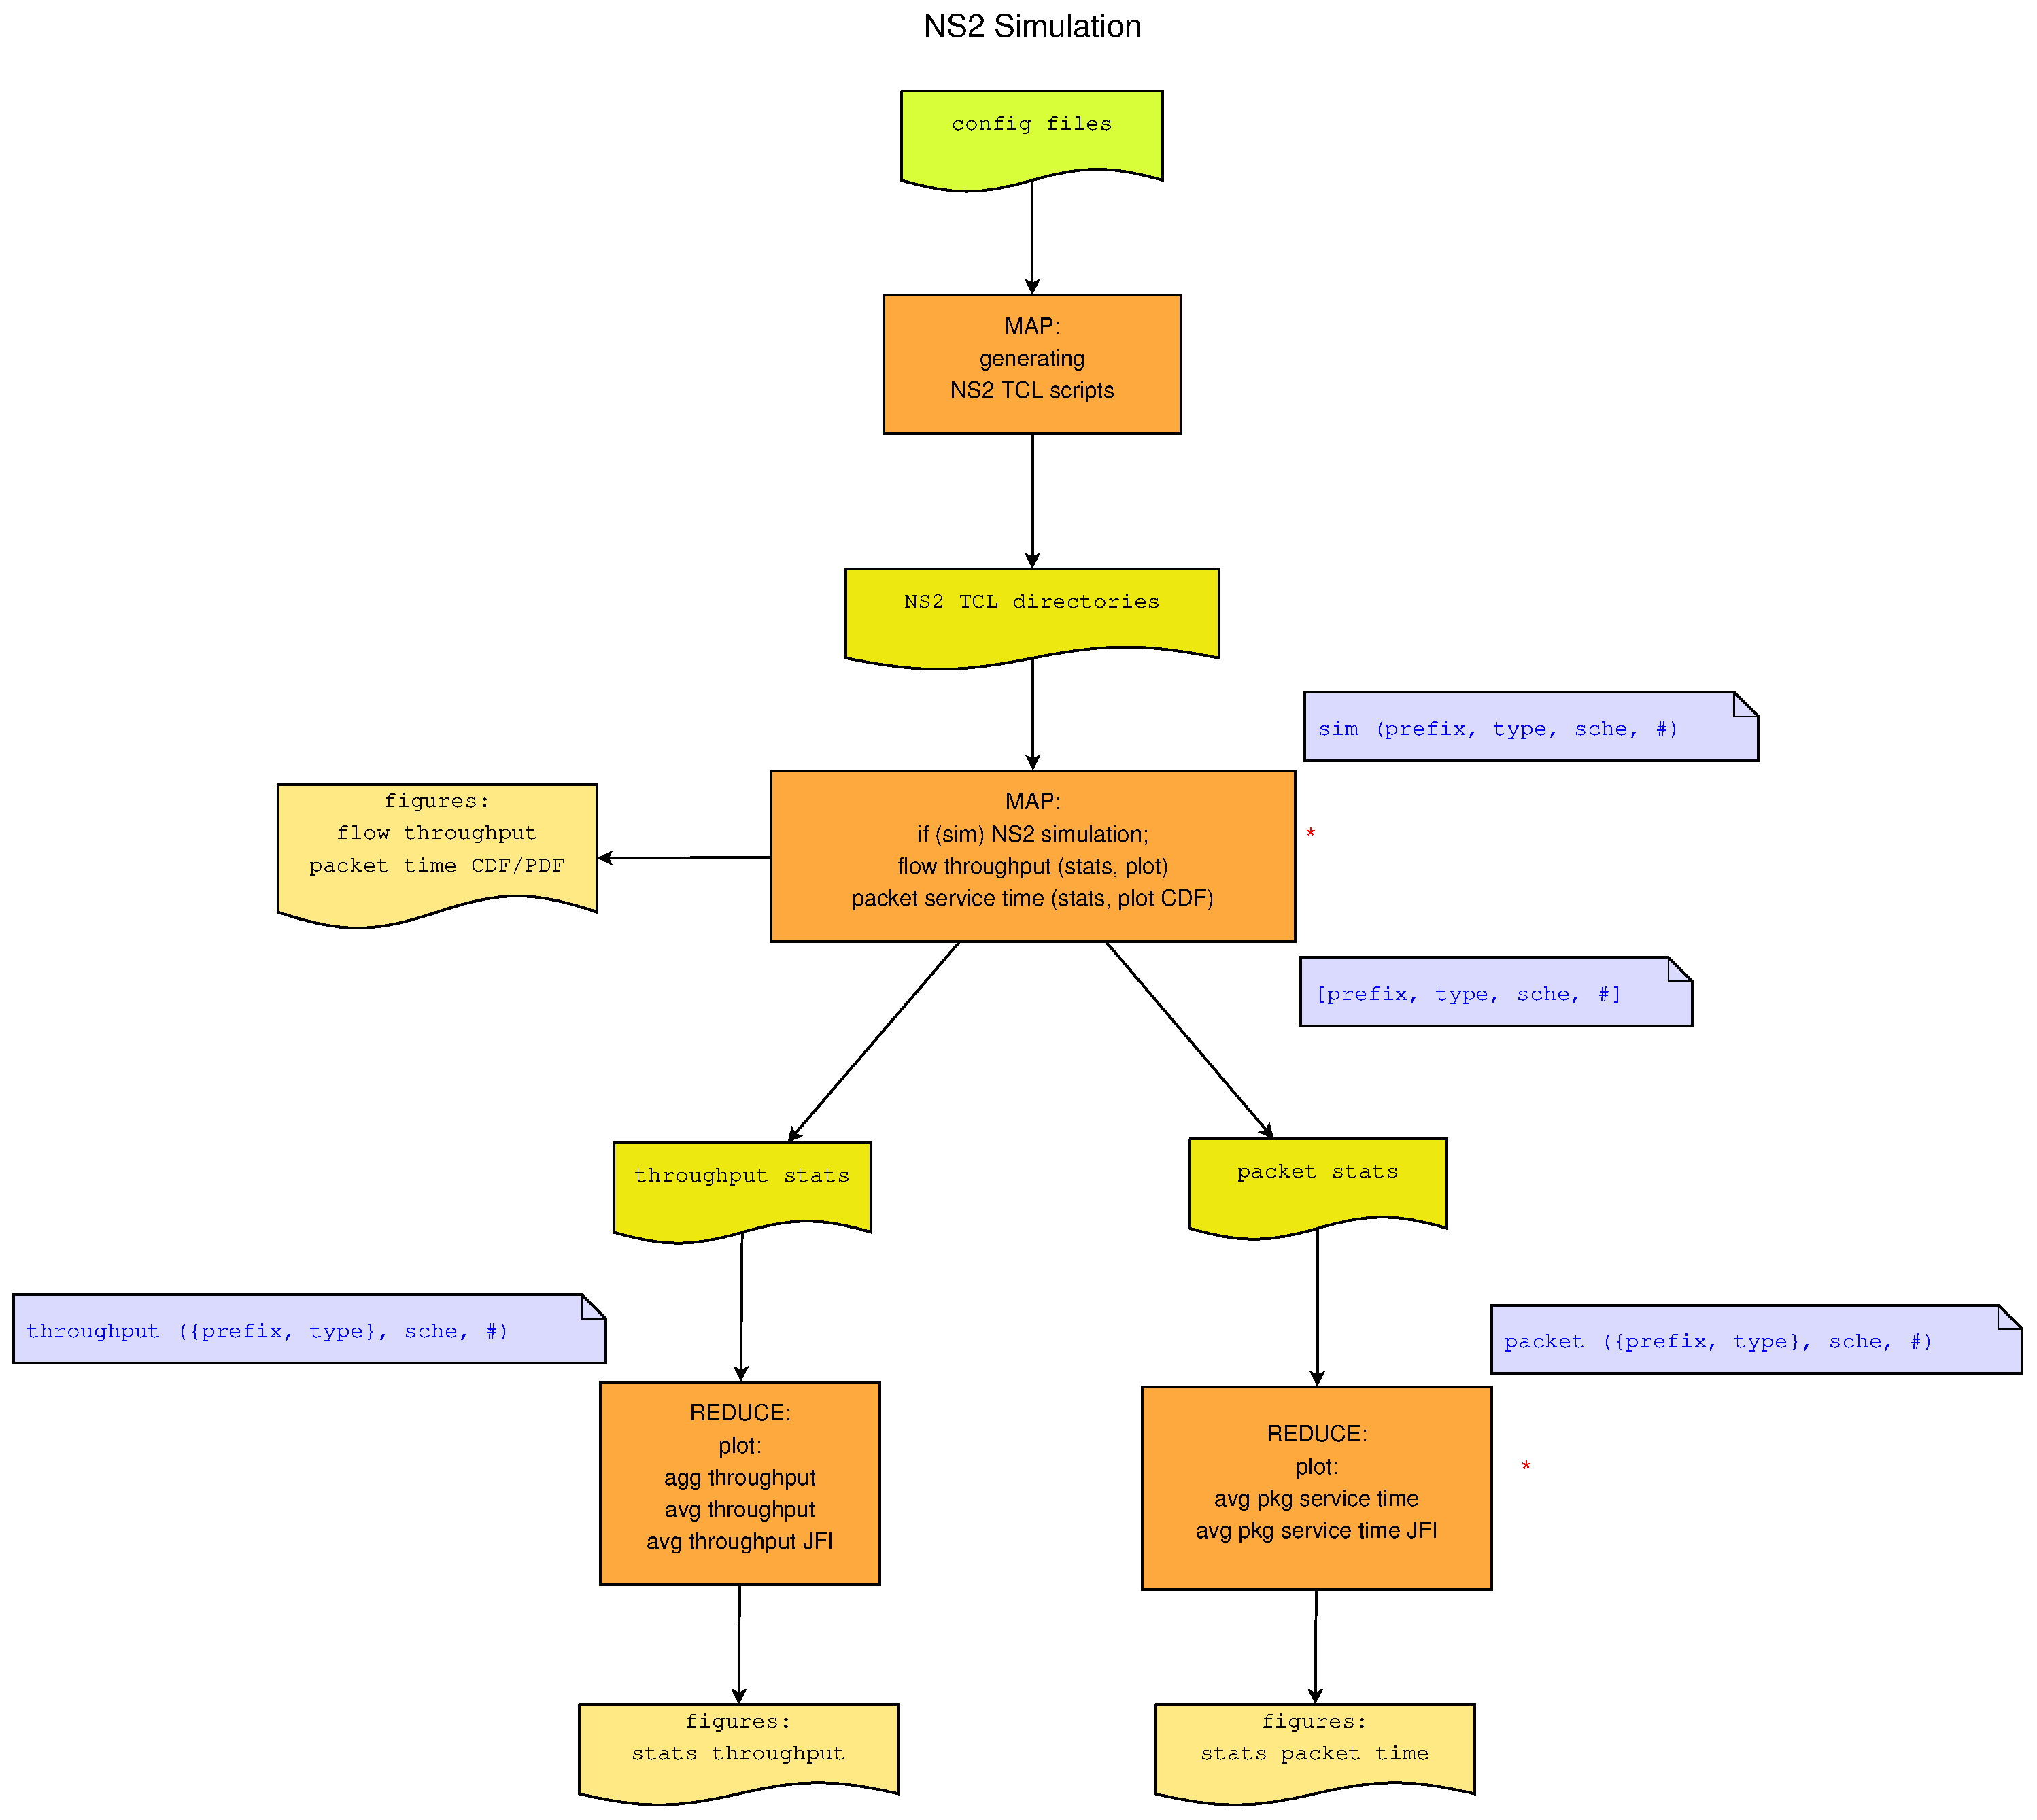
\includegraphics[width=0.9\textwidth]{flowchart-1-ns2figures}
  \caption{The system.
    The text in \fcolorbox{black}{vidtransoriginfile}{this color} is the original input file.
    The text in \fcolorbox{black}{vidtranstmpfile}{this color} is the temp file.
    The text in \fcolorbox{black}{vidtransfinalfile}{this color} is the final output file.
    The text in \fcolorbox{black}{vidtransprocess}{this color} is process block.
    The text in \fcolorbox{black}{vidtransfuncio}{\textcolor[HTML]{0000FF}{this color}} is the input/output of one process block.
The process blocks signed by a \textcolor[HTML]{FF0000}{*} are the blocks cost most of the processing time.
  }\label{fig:system}
\end{figure}

The packet delay time processing includes:
\begin{itemize}
  \item (Mgn) filter out CMTS management packets and stats
  \item (DS) filter out CMTS--CM flow and stats
  \item (US) filter out CM-CMTS flow and stats
  \item Plot DS CDF/PDF
  \item Plot Managment CDF/PDF
\end{itemize}


\chapter{Low Level Design}


\subsection{Interface of the generating configurations}

Use the streaming mode of Map-Reduce.

The input should be the config file list.


\subsubsection{map}
Function: generate directories and move and modify TCL scripts for the test.


Input parameters:
\begin{lstlisting}[language=bash]
<type> <config_file>
# config "/path/to/config.sh"
# config "/path/to/config-jjmbase.sh"
\end{lstlisting}


Output:
\begin{lstlisting}[language=bash]
<type> <prefix> <type> <scheduler> <number_of_node>
sim <prefix> <type> <scheduler> <number_of_node>
# sim  "jjmbase"  "tcp" "PF" 24
\end{lstlisting}

There should exist the directory contains the TCL scripts and data files for the simulation.





\subsection{Interface of simulation}

This stage will run the simulation base on each directory configuration,
and also generate the related throughput figures.


\subsubsection{map}
Function: run the simulations.


Input parameters:
\begin{lstlisting}[language=bash]
<type> <config_file> <prefix> <type> <scheduler> <number_of_node>
sim <config_file> <prefix> <type> <scheduler> <number_of_node>
# sim "config-xx.sh" "jjmbase"  "tcp" "PF" 24
\end{lstlisting}


Output:
\begin{lstlisting}[language=bash]
<type> <config_file> <prefix> <type> <scheduler> <number_of_node>
throughput <config_file> <prefix> <type> <scheduler> <number_of_node>
packet <config_file> <prefix> <type> <scheduler> <number_of_node>
# throughput "config-xx.sh" "jjmbase"  "tcp" "PF" 24
# packet "config-xx.sh" "jjmbase"  "tcp" "PF" 24
\end{lstlisting}

The routine should run ns2 and process stats, figures of throughput/packet.




\subsubsection{reduce}
Function: plot JFI figures


Input: (all of the columns are keys)
\begin{lstlisting}[language=bash]
<type> <config_file> <prefix> <type> <scheduler> <number_of_node>
throughput <config_file> <prefix> <type> <scheduler> <number_of_node>
packet <config_file> <prefix> <type> <scheduler> <number_of_node>
# throughput "config-xx.sh" "jjmbase"  "tcp" "PF" 24
# packet "config-xx.sh" "jjmbase"  "tcp" "PF" 24
\end{lstlisting}

Output: figures


%\input{chap-implementation.tex}

\appendix

\chapter{References}

Google MapReduce for C: Run Native Code in Hadoop
\url{http://google-opensource.blogspot.com/2015/02/mapreduce-for-c-run-native-code-in.html}



Cloud MapReduce -- A MapReduce implementation on Amazon Cloud OS
\url{https://code.google.com/p/cloudmapreduce/}


Apache Storm is a free and open source distributed realtime computation system.
\url{http://storm.apache.org/}

Apache Spark is a fast and general engine for large-scale data processing.
\url{http://spark.apache.org/}


\section{C/C++}


\href{http://hypertable.com/}{Hypertable} is a high performance, open source, massively scalable database modeled after Bigtable, Google's proprietary, massively scalable database.

\section{python}


\href{https://github.com/mfisk/filemap.git}{FileMap} is a file-based map-reduce system for data-parallel computation. (python)

\href{https://code.google.com/p/octopy/}{octopy} Easy MapReduce for Python

\href{https://github.com/michaelfairley/mincemeatpy.git}{mincemeatpy} Lightweight MapReduce in python (2013)

\href{http://heynemann.github.io/r3/}{r³} is a map reduce engine written in python using a redis backend. It's purpose is to be simple.


\href{http://discoproject.org/}{Disco} is a lightweight, open-source framework for distributed computing based on the MapReduce paradigm.



\url{https://wiki.python.org/moin/ParallelProcessing}
python Parallel Processing

\href{http://ipython.org/}{IPython} provides tools for interactive and parallel computing that are widely used in scientific computing, but can benefit any Python developer.

\section{Bash}

bashreduce (origin) \url{https://github.com/erikfrey/bashreduce.git}

improved bashreduce \url{https://github.com/dakusui/bredxbred.git},
or \url{https://github.com/rcrowley/bashreduce.git}. others, \href{https://github.com/jweslley/bashreduce.git}{jweslley}.



others:
\href{https://github.com/jasonMatney/BashMapReduce.git}{BashMapReduce},
\href{https://github.com/sorhus/bash-reduce.git}{bash-reduce},
\href{https://github.com/colestanfield/map-reduce.git}{map-reduce},
\href{https://github.com/argent0/mr-tools.git}{mr-tools},


\section{others}



\url{http://quantcast.github.io/qfs/}
Quantcast File System (QFS) is a high-performance, fault-tolerant, distributed file system developed to support MapReduce processing, or other applications reading and writing large files sequentially.

\href{https://rubygems.org/gems/mapredus}{mapredus}, simple mapreduce framework using redis and resque

\href{http://projects.camlcity.org/projects/plasma.html}{Plasma}: Distributed filesystem, key/value db, and map/reduce system. 2011


\href{http://mapreduce.sandia.gov/}{MapReduce-MPI Library} includes C++ and C interfaces callable from most hi-level languages, and also a Python wrapper


\href{http://sector.sourceforge.net/}{Sector/Sphere} is a system for distributed data storage, distribution, and processing. The system works on clusters of commodity computers. Sector provides client tools to access data stored in the system and API for the development of distributed data processing applications.

\href{http://skynet.rubyforge.org/}{Skynet} is an open source Ruby implementation of Google’s MapReduce framework


\href{https://code.google.com/p/httpmr/}{httpmr} A scalable data processing framework for people with web clusters


\href{https://code.google.com/p/qizmt/}{qizmt} is a mapreduce framework for executing and developing distributed computation applications on large clusters of Windows servers.




\href{https://code.google.com/p/cloudmapreduce/}{Cloud MapReduce} -- A MapReduce implementation on Amazon Cloud OS

\url{https://github.com/googlecloudplatform/appengine-mapreduce}
A library for running MapReduce jobs on App Engine




\url{https://github.com/documentcloud/cloud-crowd}
Write your scripts in Ruby, Works with Amazon EC2 and S3



\url{http://www.cse.ust.hk/gpuqp/Mars.html}
A MapReduce Framework on Graphics Processors


\url{https://github.com/ryanmcgrath/maprejuice}
javascript, node.js

\chapter{Source Code}

\begin{lstlisting}[language=bash]
ffprobe -show_streams
\end{lstlisting}


\end{document}



